\section{HTML Imports}\label{html-imports}

\begin{itemize}
\item
  TODO:
\item
  Vulcanize
\item
  Performance
\item
  Ausformulieren
\item
  Complete
\end{itemize}

\subsection{Einführung}\label{einfuxfchrung}

\begin{itemize}
\tightlist
\item
  Praktisch alle Plattformen erlauben es, Code zum Importieren, nur
  nicht das Web.
\item
  Bisher ist es nur möglich JavaScript, CSS, Images etc. in ein HTML
  Dokument zu importieren, HTML selbst hingegen nicht
\item
  ebenso gibt es keine Möglichkeit JavaScript, CSS, HTML, etc. via einer
  einzigen Resource zu importieren
\item
  HTML Imports sollen dieses Problem lösen
\end{itemize}

\subsection{HTML importieren}\label{html-importieren}

\begin{itemize}
\tightlist
\item
  HTML Imports werden, wie andere Imports auch, per
  \texttt{\textless{}link\textgreater{}} Tag deklariert
\item
  Als \texttt{rel} Attribut wird ``import'' angegeben
\end{itemize}

\begin{Shaded}
\begin{Highlighting}[]
\KeywordTok{<head>}
  \KeywordTok{<link}\OtherTok{ rel=}\StringTok{"import"}\OtherTok{ href=}\StringTok{"/imports/myimport.html"}\KeywordTok{>}
\KeywordTok{</head>}
\end{Highlighting}
\end{Shaded}

\begin{itemize}
\tightlist
\item
  Ein HTML Import wird nur einmal geladen, auch wenn ein Request auf
  eine HTML Datei mehrmals erfolgt, d.h. enthaltenes JavaScript wird nur
  einmal ausgeführt
\item
  HTML Imports von einer anderen Domain sind eine Sicherheitslücke, wenn
  man aber dennoch eine HTML Datei von einer anderen Seite importieren
  will, muss CORS (Cross Origin Resource Sharing) aktiviert sein
  {[}Developing Web Components 2015{]}
\end{itemize}

\begin{quote}
Using only one URL, you can package together a single relocatable bundle
of web goodness for others to consume. {[}Eric Bidelman 2013{]}
\end{quote}

\subsection{Vorteil}\label{vorteil}

\begin{itemize}
\tightlist
\item
  HTML Imports ermöglichen es eine gesamte App via HTML Import zu
  importieren
\item
  So kann beispielsweise das Einbinden von Bootstrap stark vereinfacht
  werden
\end{itemize}

Bisher:

\begin{Shaded}
\begin{Highlighting}[]
\KeywordTok{<link}\OtherTok{ rel=}\StringTok{"stylesheet"}\OtherTok{ href=}\StringTok{"bootstrap.css"}\KeywordTok{>}
\KeywordTok{<link}\OtherTok{ rel=}\StringTok{"stylesheet"}\OtherTok{ href=}\StringTok{"fonts.css"}\KeywordTok{>}
\KeywordTok{<script}\OtherTok{ src=}\StringTok{"jquery.js"}\KeywordTok{></script>}
\KeywordTok{<script}\OtherTok{ src=}\StringTok{"bootstrap.js"}\KeywordTok{></script>}
\KeywordTok{<script}\OtherTok{ src=}\StringTok{"bootstrap-tooltip.js"}\KeywordTok{></script>}
\KeywordTok{<script}\OtherTok{ src=}\StringTok{"bootstrap-dropdown.js"}\KeywordTok{></script>}
\end{Highlighting}
\end{Shaded}

\begin{itemize}
\tightlist
\item
  Stattdessen kann dieses Markup nun in ein einziges HTML Dokument,
  welches alle Abhängigkeiten verwaltet, geschrieben werden
\item
  Dieses wird dann mit einem einzigen Import in das eigene HTML Dokument
  importiert
\end{itemize}

HTML Import:

\begin{Shaded}
\begin{Highlighting}[]
\KeywordTok{<head>}
  \KeywordTok{<link}\OtherTok{ rel=}\StringTok{"import"}\OtherTok{ href=}\StringTok{"bootstrap.html"}\KeywordTok{>}
\KeywordTok{</head>}
\end{Highlighting}
\end{Shaded}

\subsection{HTML Imports verwenden}\label{html-imports-verwenden}

\begin{itemize}
\tightlist
\item
  Importierte HTML Dateien werden nicht nur in das Dokument eingefügt,
  sondern vom Parser verarbeitet, das bedeutet, dass mit JavaScript auf
  den DOM des Imports zugegriffen werden kann
\item
  Um auf den Inhalt des Imports zuzugreifen muss die \texttt{.import}
  Eigenschaft des \texttt{\textless{}link\textgreater{}} zugegriffen
  werden
  \texttt{var\ content\ =\ document.querySelector(\textquotesingle{}link{[}rel="import"{]}\textquotesingle{}).import;}
\item
  Nun kann auf den DOM des \texttt{content} zugegriffen werden.
  Beispielsweise kann ein Element mit der Klasse \texttt{.element}
  geklont und dann in das eigene HTML eingefügt werden
\end{itemize}

\begin{Shaded}
\begin{Highlighting}[]
\KeywordTok{<head>}
  \KeywordTok{<link}\OtherTok{ rel=}\StringTok{"import"}\OtherTok{ href=}\StringTok{"element.html"}\KeywordTok{>}
\KeywordTok{</head>}
\KeywordTok{<body>}
  \KeywordTok{<script>}
    \KeywordTok{var} \NormalTok{content }\OperatorTok{=} \VariableTok{document}\NormalTok{.}\AttributeTok{querySelector}\NormalTok{(}\StringTok{'link[rel="import"]'}\NormalTok{).}\AttributeTok{import}\OperatorTok{;}

    \KeywordTok{var} \NormalTok{el }\OperatorTok{=} \VariableTok{content}\NormalTok{.}\AttributeTok{querySelector}\NormalTok{(}\StringTok{'.element'}\NormalTok{)}\OperatorTok{;}

    \VariableTok{document}\NormalTok{.}\VariableTok{body}\NormalTok{.}\AttributeTok{appendChild}\NormalTok{(}\VariableTok{el}\NormalTok{.}\AttributeTok{cloneNode}\NormalTok{(}\KeywordTok{true}\NormalTok{))}\OperatorTok{;}
  \OperatorTok{<}\SpecialStringTok{/script>}
\SpecialStringTok{</body}\OperatorTok{>}
\end{Highlighting}
\end{Shaded}

\subsection{Abhängigkeiten verwalten und
Sub-Imports}\label{abhuxe4ngigkeiten-verwalten-und-sub-imports}

\subsubsection{Sub-Imports}\label{sub-imports}

\begin{itemize}
\tightlist
\item
  HTML Dateien die in einem HTML Dokument importiert werden, können
  selbst auch HTML Dateien importieren
\item
  Somit können andere Komponenten wiederverwendet und erweitert werden
\item
  Wenn eine Komponente A eine Abhängigkeit von einer Komponenten B hat
  und es eine neue Version von Komponente B gibt, kann diess einfach in
  dem Import des Sub-Imports angepasst werden ohne JavaScript ändern zu
  müssen
\end{itemize}

\subsubsection{Abhänigkeiten
verwalten}\label{abhuxe4nigkeiten-verwalten}

\begin{itemize}
\tightlist
\item
  Wenn mehrere HTML Imports die gleichen Abhängigkeiten - z.B. jQuery -
  haben, wird das jQuery.js dennoch automatisch nur einmal vom Browser
  heruntergeladen
\end{itemize}

index.html

\begin{Shaded}
\begin{Highlighting}[]
\KeywordTok{<link}\OtherTok{ rel=}\StringTok{"import"}\OtherTok{ href=}\StringTok{"component1.html"}\KeywordTok{>}
\KeywordTok{<link}\OtherTok{ rel=}\StringTok{"import"}\OtherTok{ href=}\StringTok{"component2.html"}\KeywordTok{>}
\end{Highlighting}
\end{Shaded}

component1.html

\begin{Shaded}
\begin{Highlighting}[]
\KeywordTok{<script}\OtherTok{ src=}\StringTok{"jQuery.html"}\KeywordTok{></script>}
\end{Highlighting}
\end{Shaded}

component2.html

\begin{Shaded}
\begin{Highlighting}[]
\KeywordTok{<script}\OtherTok{ src=}\StringTok{"jQuery.html"}\KeywordTok{></script>}
\end{Highlighting}
\end{Shaded}

jQuery.html

\begin{Shaded}
\begin{Highlighting}[]
\KeywordTok{<script}\OtherTok{ src=}\StringTok{"js/jquery.js"}\KeywordTok{></script>}
\end{Highlighting}
\end{Shaded}

\begin{itemize}
\tightlist
\item
  Des Weiteren muss auch nicht auf die Reihenfolge der Imports geachtet
  werden, da diese selbst ihre Abhängigkeiten beinhalten
\end{itemize}

{[}Eiji Kitamura 2015{]}

\subsection{Performance - TODO}\label{performance---todo}

\begin{quote}
Sind Web Components nicht eine Katastrophe für die Performance? So
spaltet sich doch die komplette Seite in hundert Einzel-Downloads auf,
jede Komponente lädt jedes Mal neu jQuery \ldots{} oder gibt es da einen
Trick?
\end{quote}

\begin{quote}
Heutzutage ist das möglicherweise tatsächlich ein Problem, das sich aber
in Zukunft von selbst in Luft auflösen wird. Das Doppel-Download-Problem
besteht in Browsern mit nativer Unterstützung für Web Components gar
nicht erst, da hier Doppel-Requests automatisch dedupliziert werden (so
liest man jedenfalls allerorten; in konkreten Specs habe ich nichts
gefunden, das das verlangt). Im Polymer-Polyfill passiert das einfach
anhand des Ressourcen-Pfades, die native Implementierung soll auch
identische Ressourcen aus unterschiedlichen Quellen deduplizieren
können.
\end{quote}

\begin{quote}
Dass Web Components dann immer noch zu vielen Einzel-Requests führen,
ist in nicht all zu ferner Zukunft ein Feature und kein Bug. Mit HTTP/2
bzw. SPDY als Netzwerkprotokoll hat man, anders als beim HTTP 1.1 von
heute, keinen Vorteil mehr, wenn man Ressourcen zusammenfasst. Im
Gegenteil: wenn man sein Frontend in viele kleine Teile aufsplittet, hat
man den Vorteil, dass bei der Änderung einer einzigen Icongrafik der
Nutzer nicht mehr das komplette Bild-Sprite, sondern wirklich nur eine
einzige Winzdatei neu herunterladen muss. Anders gesagt übernimmt HTTP/2
das Zusammenfassen von Dateien auf Protokollebene und Webentwickler
müssen es nicht mehr selbst machen. Und nur die üblichen Verdächtigen
(d.h. IE und Safari) können das nicht bereits heute. Mehr Infos zum
Thema gibt es in einem epischen Slide Deck aus der Feder von
Performance-Papst Schepp.
\end{quote}

\begin{quote}
Die Web-Component-Performance-Problematik löst sich also im Laufe der
Zeit von selbst. Bis dahin kann man sich mit \emph{Vulcanize}, einem
Tool zum Zusammenfassen von HTML-Imports inklusive aller Ressourcen in
eine einzige Datei, behelfen.
\end{quote}

{[}Peter Kröner 2014{]}

\subsubsection{HTTP/2 - TODO}\label{http2---todo}

\subsubsection{\texorpdfstring{``Vulcanize'' -
TODO}{Vulcanize - TODO}}\label{vulcanize---todo}

\subsection{Anwendungen}\label{anwendungen}

\begin{itemize}
\tightlist
\item
  Ganze Web Applikationen mit HTML/JavaScript/CSS können in eine Datei
  geschrieben und von anderen Importiert werden
\item
  Code Organisation: Einzelne Abschnitte einer Anwendung oder von Code
  können in einzelne Dateien ausgelagert werden, was Web Applikationen
  modular und wiederverwendbar macht
\item
  HTML Imports können ein oder mehrere Custom Elements beinhalten und in
  eine Applikation einbinden. Somit wird das Interface des Elements und
  dessen Definition gekapselt
\item
  Abhängigkeitsverwaltung: Resourcen werden automatisch nur einmal
  geladen
\item
  Einzelne kleine JavaScripts werden schneller ausgeführt als wenn der
  Browser eine große JavaScript Library parsen und dann ausführen muss
\end{itemize}

{[}Eric Bidelman 2013{]}

\subsection{Browserunterstüzung}\label{browserunterstuxfczung}

\begin{itemize}
\tightlist
\item
  HTML Imports wurden noch nicht vom W3C standardisiert, sondern sind
  noch ein Working Draft (http://www.w3.org/TR/html-imports/)
\item
  Deshalb werden sie bisher auch nur in Chrome und Opera unterstützt
\end{itemize}

\begin{figure}[htbp]
\centering
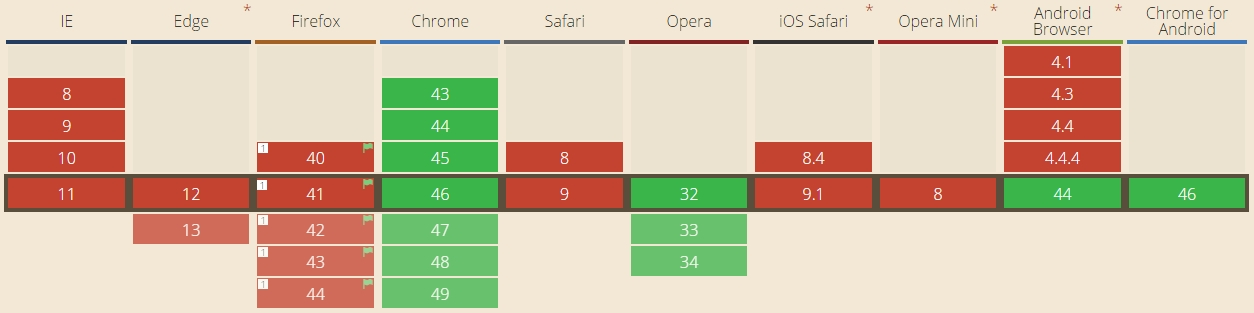
\includegraphics{images/4-html-imports-browserunterstuetzung.jpg}
\caption{Bild: HTML Imports Browserunterstützung}
\end{figure}

{[}Can I Use 2015{]}

\subsection{Quellen}\label{quellen}

\begin{itemize}
\tightlist
\item
  {[}Developing Web Components 2015{]} Jarrod Overson \& Jason Strimpel,
  Developing Web Components, O'Reilly 2015, S.139-147
\item
  {[}Eric Bidelman 2013{]}
  http://www.html5rocks.com/en/tutorials/webcomponents/imports/
\item
  {[}Can I Use 2015{]} Can I Use, http://caniuse.com/\#search=imports
\item
  http://www.w3.org/TR/html-imports/
\item
  {[}Peter Kröner 2014{]} Peter Kröner,
  http://www.peterkroener.de/fragen-zu-html5-und-co-beantwortet-15-web-components-performance-css-variablen-data-urls-async/
\item
  http://www.hongkiat.com/blog/html-import/
\item
  {[}Eiji Kitamura 2015{]} Eiji Kitamura, Introduction to HTML Imports,
  http://webcomponents.org/articles/introduction-to-html-imports/
\end{itemize}
